\documentclass[journal]{IEEEtran}
\usepackage[a5paper, margin=10mm, onecolumn]{geometry}
%\usepackage{lmodern} % Ensure lmodern is loaded for pdflatex
\usepackage{tfrupee} % Include tfrupee package

\setlength{\headheight}{1cm} % Set the height of the header box
\setlength{\headsep}{0mm}     % Set the distance between the header box and the top of the text

\usepackage{gvv-book}
\usepackage{gvv}
\usepackage{cite}
\usepackage{amsmath,amssymb,amsfonts,amsthm}
\usepackage{algorithmic}
\usepackage{graphicx}
\usepackage{textcomp}
\usepackage{xcolor}
\usepackage{txfonts}
\usepackage{listings}
\usepackage{enumitem}
\usepackage{mathtools}
\usepackage{gensymb}
\usepackage{comment}
\usepackage[breaklinks=true]{hyperref}
\usepackage{tkz-euclide} 
\usepackage{listings}
% \usepackage{gvv}                                        
\def\inputGnumericTable{}                                 
\usepackage[latin1]{inputenc}                                
\usepackage{color}                                            
\usepackage{array}                                            
\usepackage{longtable}                                       
\usepackage{calc}                                             
\usepackage{multirow}                                         
\usepackage{hhline}                                           
\usepackage{ifthen}                                           
\usepackage{lscape}
\begin{document}

\bibliographystyle{IEEEtran}
\vspace{3cm}

\title{10.3.2.3.3}
\author{EE24BTECH11064 - Harshil Rathan}
 \maketitle
% \newpage
% \bigskip
{\let\newpage\relax\maketitle}

\renewcommand{\thefigure}{\theenumi}
\renewcommand{\thetable}{\theenumi}
\setlength{\intextsep}{10pt} % Space between text and floats


\numberwithin{equation}{enumi}
\numberwithin{figure}{enumi}
\renewcommand{\thetable}{\theenumi}
\textbf{Question}:\\
On comparing the ratios $\frac{a_1}{a_2}$, $\frac{b_1}{b_2}$ and $\frac{c_1}{c_2}$ find out whether the following pair of linear equations are consistent, or inconsistent. 
\begin{align*}
    \frac{3}{2}x+\frac{5}{3}y = 7 \\ 9x+10y = 14 
\end{align*}
\\
\textbf{Solution: }\\
The general form of a pair of linear equations is given as:
\begin{align*}
    a_1x + b_1y  = c_1 \\
    a_2x + b_2y = c_2
\end{align*}
Here, the coefficients are:
\begin{align*}
    a_1 = \frac{3}{2}, \quad b_1 = \frac{5}{3}, \quad c_1 = 7, \\
    a_2 = 9, \quad b_2 = 10, \quad c_2 = 14.
\end{align*}
We calculate the ratios:
\begin{align*}
    \frac{a_1}{a_2} = \frac{1}{6}, \quad \frac{b_1}{b_2} = \frac{1}{6}, \quad \frac{c_1}{c_2} = \frac{1}{2}.
\end{align*}
Since $\frac{a_1}{a_2} = \frac{b_1}{b_2} \neq \frac{c_1}{c_2}$ , the given system of equations is inconsistent.\\
\textbf{Solution using LU Decomposition}\\
Simplifying and using matrix notation,
\begin{align}
    \frac{3}{2}x+\frac{5}{3}y = 7\\
    9x+10y = 14\\
    \myvec{
        \frac{3}{2} & \frac{5}{3}\\
        9 & 10
    } \myvec{x \\ y}= \myvec{ 7\\ 14}
\end{align}

Any non-sigular matrix can be represented as a product of a lower triangular matrix $L$ and an
upper triangular matrix $U$

\begin{align}
    A\vec{x} = LU\vec{x} = \vec{b}
\end{align}
The upper triangular matrix U is found by row reducing A,
\begin{align}
    \myvec{
        \frac{3}{2} & \frac{5}{3}\\
        9 & 10
    } \xrightarrow{R_2 -> R_2 -  6 R_1}  \myvec{
        \frac{3}{2} & \frac{5}{3}\\
        0 & 0
    } 
\end{align}
Let 
\begin{align}
    L = \myvec{1 & 0\\ l_{21} & 1}
\end{align}
$l_{21}$ is the multiplier used to zero $a_{21}$, so $l_{21} = 6$.\\
\newline
Now,
\begin{align}
   A =  \myvec{
        \frac{3}{2} & \frac{5}{3}\\
        9 & 10
    } = \myvec{1 & 0\\ 6 & 1} \myvec{\frac{3}{2} & \frac{5}{3} \\ 0 & 0 }
\end{align}
Now we can get the solution to our problem by the two step process,
\begin{align}
    L\vec{y} = \vec{b}\\
    U\vec{x} = \vec{y}
\end{align}
Using forward substitution to solve the first equation,
\begin{align}
    \myvec{1 & 0 \\ 6 & 1}\myvec{y_1 \\ y_2} &= \myvec{7 \\ 14}\\
    \xrightarrow{} \myvec{y_1 \\ y_2} &= \myvec{7 \\ -28} 
\end{align}
Now using back-substitution for the second equation,
\begin{align}
    \myvec{\frac{3}{2} & \frac{5}{3} \\ 0 & 0 }\myvec{x_1 \\ x_2} &= \myvec{7 \\ -28} \\
    \myvec{x_1 \\ x_2} &= \myvec{ ? \\ ?}
\end{align}
The equation gives 
\begin{align}
    0 = -28 
\end{align}
Which is a contradiction \\
This means that the system is inconsistent and has no solution. Therefore, there is no solution for $x_1$ and $x_2$ \\
\textbf{Numerical Computation for LU Decomposition}\\
We want to decompose A as the product of a lower triangular matrix L and an upper triangular matrix U  
\begin{align}
    A = LU
\end{align}
L is a lower triangular matrix with ones on the diagonal
\begin{align}
    L = \myvec{1 & 0 & 0 & \cdots & 0 \\
L_{21} & 1 & 0 & \cdots & 0 \\
L_{31} & L_{32} & 1 & \cdots & 0 \\
\vdots & \vdots & \vdots & \ddots & \vdots \\
L_{n1} & L_{n2} & L_{n3} & \cdots & 1}
\end{align}
U is an upper triangular matrix
\begin{align}
    \myvec{U_{11} & 0 & 0 & \cdots & 0 \\
U_{12} & U_{22} & 0 & \cdots & 0 \\
U_{13} & U_{23} & U_{33} & \cdots & 0 \\
\vdots & \vdots & \vdots & \ddots & \vdots \\
U_{1n} & U_{2n} & U_{3n} & \cdots & U_{nn}}
\end{align}
The first row of $U$ is simply the first row of $A$
\begin{align}
    U_{1j} = A_{1j} 
\end{align}
The first column of $L$ is computed as
\begin{align}
    L_{i1} = \frac{A_{i1}}{U_{11}}, \quad \text{for} \quad i = 2, 3, \dots, n.
\end{align}
Subsequent columns of $U$ are computed as 
\begin{align}
    U_{kj} = A_{kj} - \sum_{m=1}^{k-1} L_{km} U_{mj}
\end{align}
for $j = k, k+1, \dots, n$\\
Subsequent columns of $L$ are computed as
\begin{align}
    L_{ik} = \frac{A_{ik} - \sum_{m=1}^{k-1} L_{im} U_{mk}}{U_{kk}}
\end{align}
for $i= k+1, k+2, \dots, n$ \\
This systematic approach ensures that the matrix \( A \) is decomposed into \( L \) and \( U \) 
\begin{figure}[h!]
   \centering
   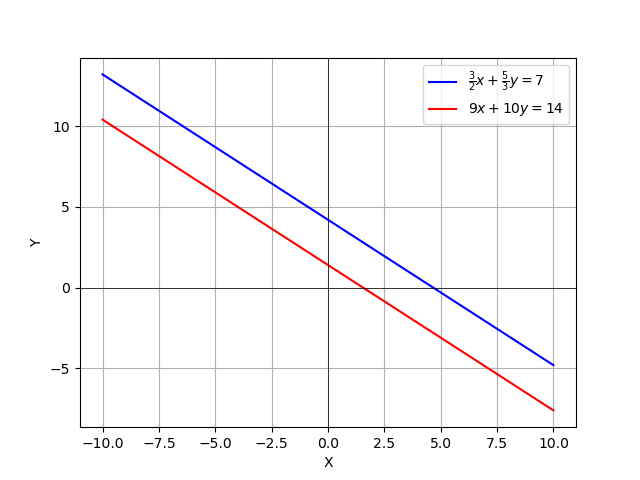
\includegraphics[width=\columnwidth]{figs/Figure_1.png}
\end{figure}
\end{document}
